%&tex
\chapter{Disentangling Generative Factors}
	% POSE APPEARANCE SWAP
	\begin{figure}[t]
		\centering
		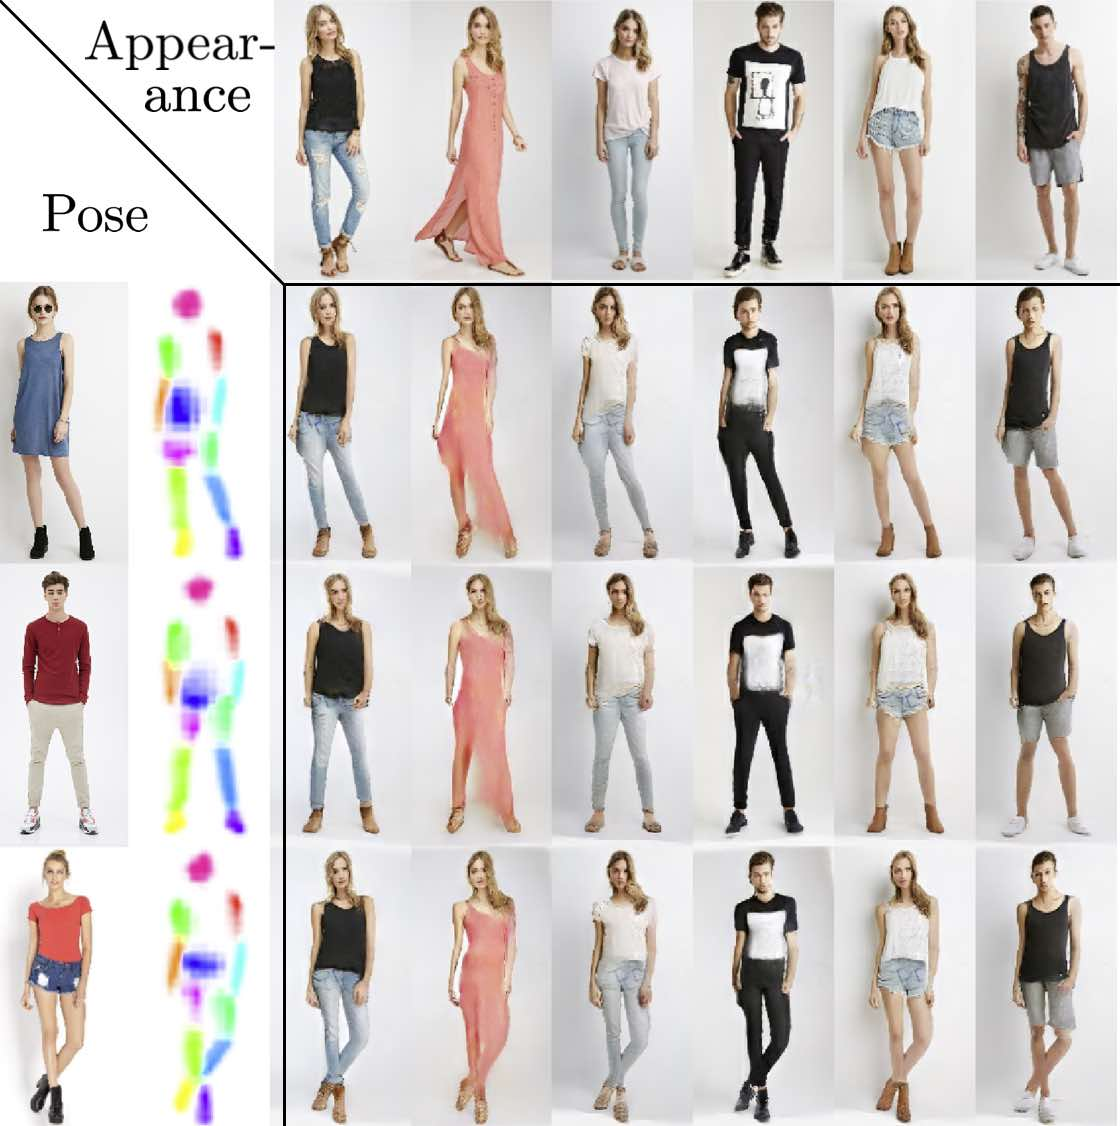
\includegraphics[trim={0cm 0cm 0cm 0cm},clip, width=.5\linewidth]{fig/factor/swappy}
		\caption{Transferring shape and appearance on Deep Fashion. Without annotation the model estimates shape, 2nd column. Target appearance is extracted from images in top row to synthesize images. Note that we trained without image pairs only using synthetic transformations.
		%for training we had no image pairs but only synthetic transformations.
		%without being explicitly trained for this task.
		All images are from the test set.}
		\label{fig:allswaps}
	\end{figure}

	\begin{table}
		\centering
		\caption{Mean average precision (mAP) and rank-n accuracy for person re-identification on synthesized images after performing shape/appearance swap. Input images from Deep Fashion test set. Note \cite{esser18} is supervised \wrt shape.}
		\label{tab:reid}
		\begin{tabular}{l|cccr}
			\hline
			& mAP & rank-1 & rank-5 & rank-10 \\ \hline
			VU-Net \cite{esser18} & 88.7\% & 87.5\% & {98.7}\% & {99.5}\% \\
			Ours & {90.3}\% & {89.4}\% &{98.2}\% & {99.2}\% \\ \hline
		\end{tabular}
	\end{table}

	\begin{table}
		\centering
		\caption{Percentage of Correct Keypoints (PCK) for pose estimation on shape/appearance swapped generations.\;$\alpha$ is pixel distance divided by image diagonal. Note that \cite{esser18} serves as upper bound, as it uses the groundtruth shape estimates.}
		%shape supervision.}
		\label{tab:pose}
		\begin{tabular}{l|cccr}
			\hline
			$\alpha$ & $2.5\%$ &  $5\%$ & $7.5\%$ & $10\%$ \\ \hline
			VU-Net \cite{esser18} & {95.2}\% & {98.4}\% & {98.9}\% & {99.1}\% \\
			Ours & 85.6\% & 94.2\% &96.5\% & 97.4\% \\ \hline
		\end{tabular}
	\end{table}

	Disentangled representations of object shape and appearance allow to alter both properties individually to synthesize new images. The ability to flexibly control the generator allows, for instance, to change the pose of a person or their clothing. In contrast to previous work \cite{esser18, denton17disvideo, ma17poseguided, ma17disperson, debem18dgpose, jakab18},
	we achieve this ability without requiring supervision \textit{and} using a flexible part-based model instead of a holistic representation. This allows to explicitly control the parts of an object that are to be altered. We quantitatively compare against \emph{supervised} state-of-the-art disentangled synthesis of human figures. Also we qualitatively evaluate our model on unsupervised synthesis of still images, video-to-video translation, and local editing for appearance transfer.
	% \todo{t-SNE of Shape Representation, t-SNE of Appearance Representation}

	\section{Disentangling Pose and Appearance}

	\paragraph{Deep Fashion} \cite{liu16deepfashion, liu16deepfashionwild} consists of ca. 53k in-shop clothes images in high-resolution of $256 \times 256$. We selected the images which are showing a full body (all keypoints visible, measured with the pose estimator by \cite{cao17affinityfield}) and used the provided train-test split. For comparison with Esser \etal \cite{esser18} we used their published code.

	On Deep Fashion \cite{liu16deepfashion, liu16deepfashionwild}, a benchmark dataset for supervised disentangling methods, the task is to separate person ID (appearance) from body pose (shape) and then synthesize new images for previously unseen persons from the test set in eight different poses. We randomly sample the target pose and appearance conditioning from the test set. Fig. \ref{fig:allswaps} shows qualitative results.
	We quantitatively compare against supervised state-of-the-art disentangling \cite{esser18} by evaluating \emph{i)} invariance of appearance against variation in shape by the re-identification error and \emph{ii)} invariance of shape against variation in appearance by the distance in pose between generated and pose target image.

	\subsection{Person Re-Identification}
	% \begin{itemize}
		% \item t-SNE of IDs
		% \item Own, Other (stronger statement)
	% \end{itemize}
	\note{reid more, for us only means}

	\begin{figure}[htp]
		\centering
		\begin{subfigure}{0.49\linewidth}
		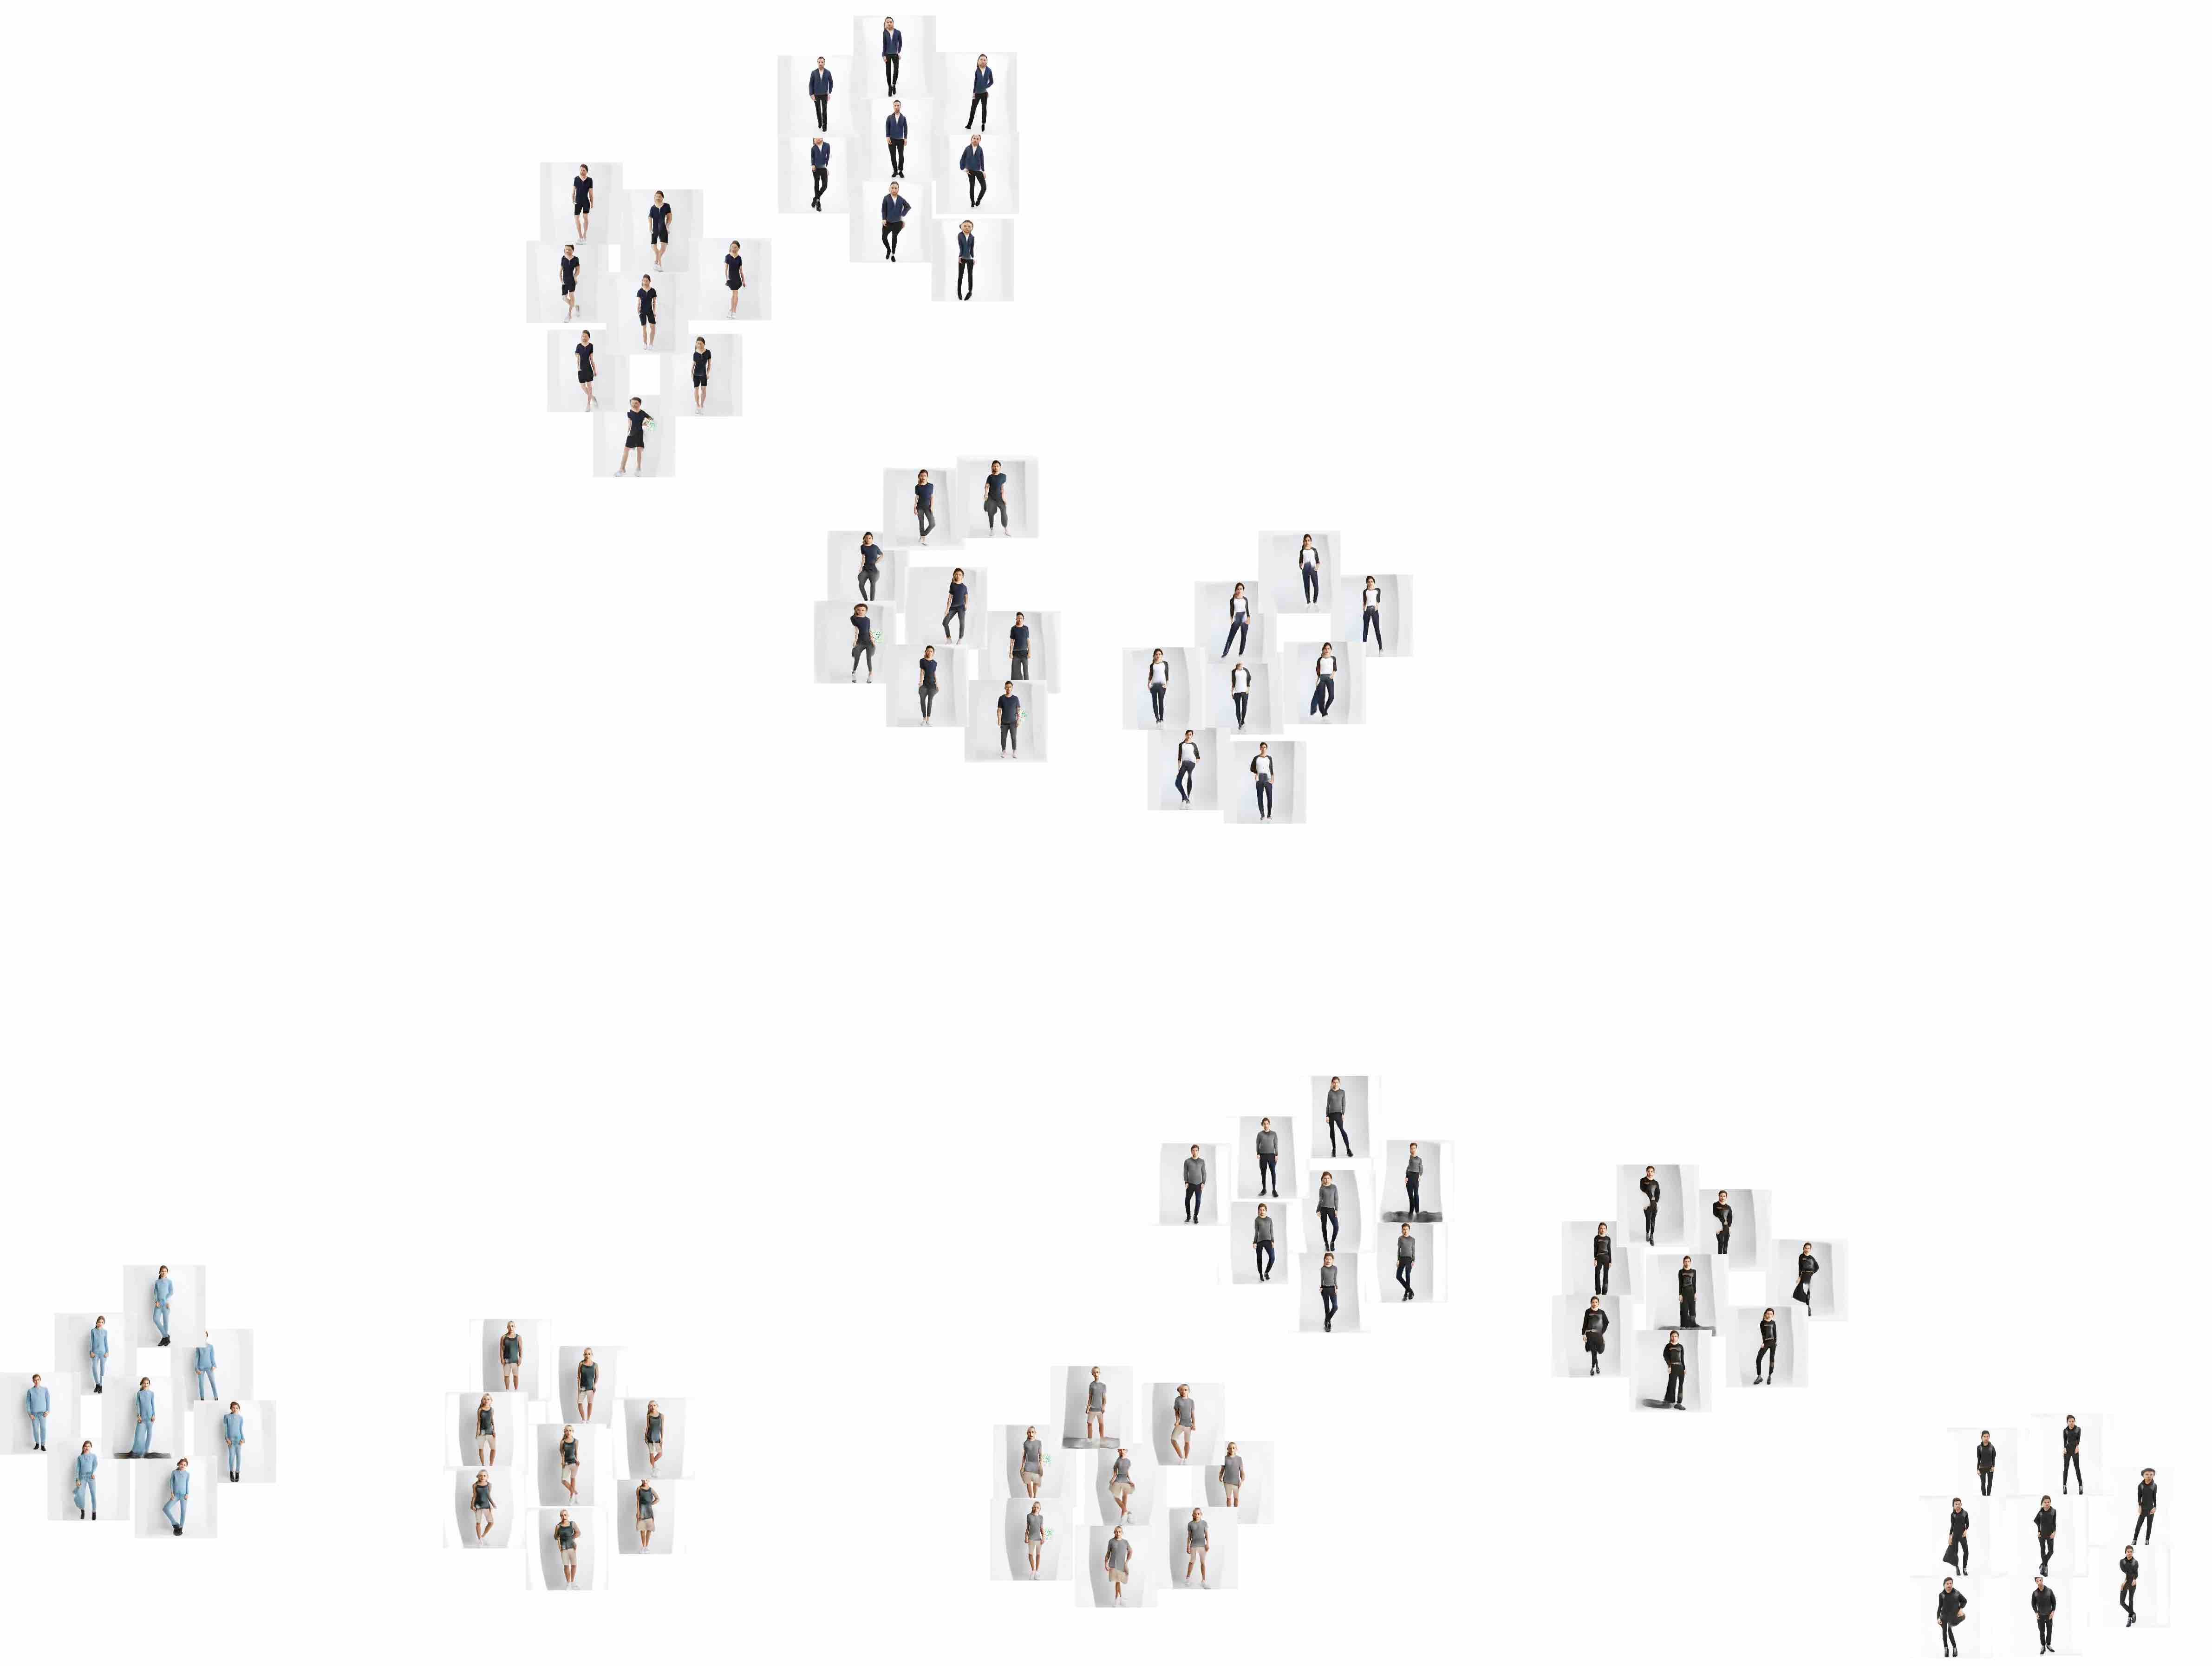
\includegraphics[trim={0cm 0cm 0cm 0cm},clip, width=1.0\linewidth]{fig/factor/tsne_img}
		\end{subfigure}
		\begin{subfigure}{0.49\linewidth}
		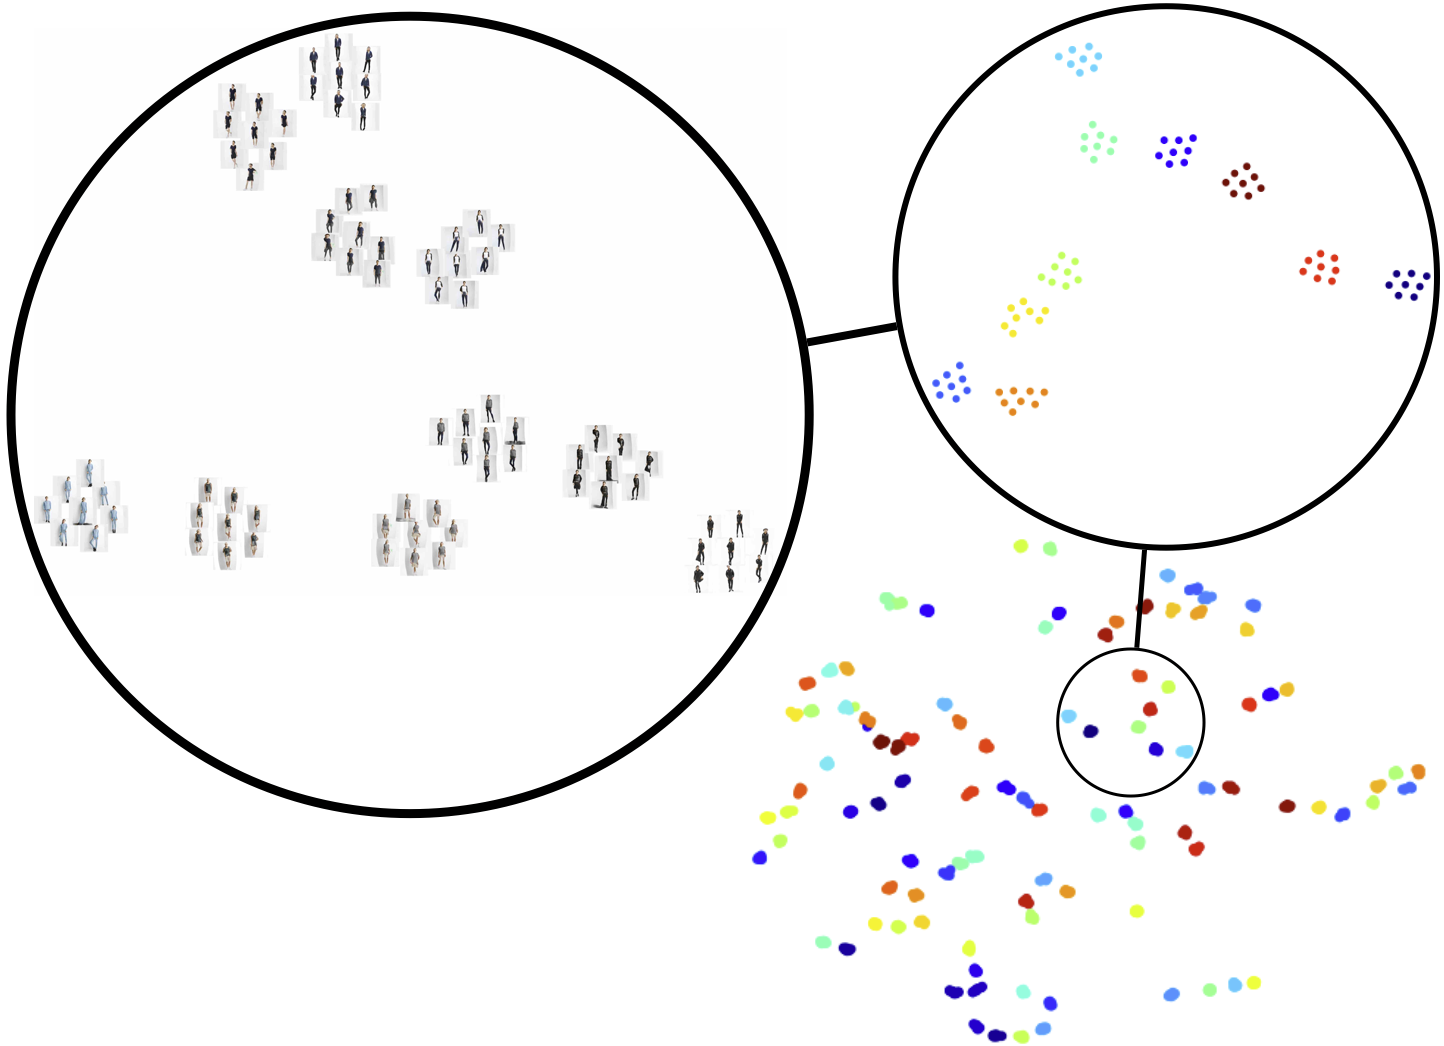
\includegraphics[trim={0cm 0cm 0cm 0cm},clip, width=1.0\linewidth]{fig/factor/tsne_bubble}
		\end{subfigure}
		% \begin{subfigure}{0.49\linewidth}
			% % \begin{subfigure}{0.49\linewidth}
			% 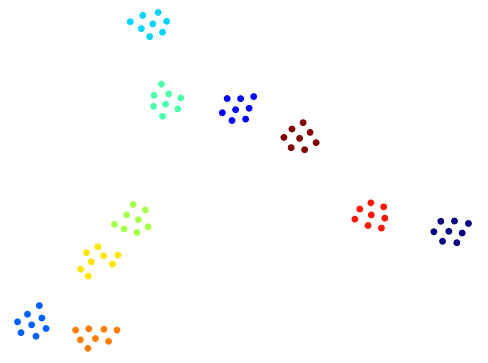
\includegraphics[trim={0cm 0cm 0cm 0cm},clip, width=1.0\linewidth]{fig/factor/tsne10}
			% \end{subfigure}\begin{subfigure}{0.49\linewidth}
			% 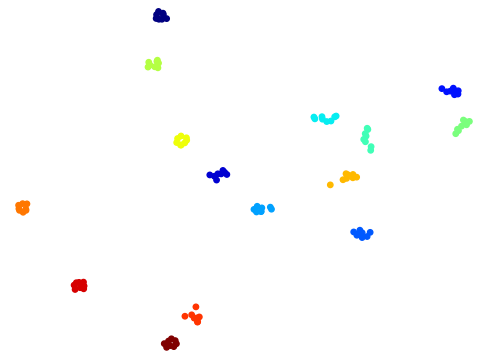
\includegraphics[trim={0cm 0cm 0cm 0cm},clip, width=1.0\linewidth]{fig/factor/tsne15}
			% \end{subfigure}
%
			% \begin{subfigure}{0.49\linewidth}
			% 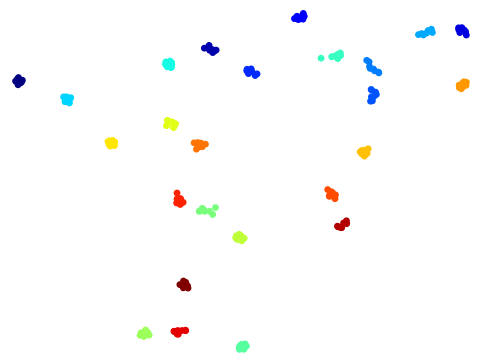
\includegraphics[trim={0cm 0cm 0cm 0cm},clip, width=1.0\linewidth]{fig/factor/tsne20}
			% \end{subfigure}
			% \begin{subfigure}{0.49\linewidth}
			% 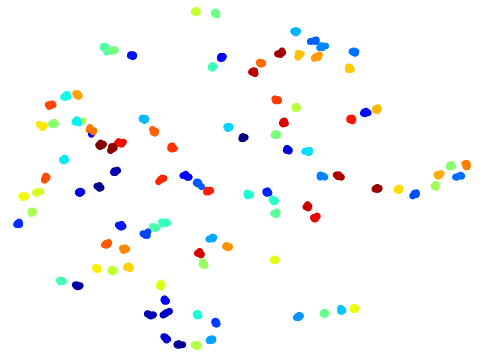
\includegraphics[trim={0cm 0cm 0cm 0cm},clip, width=1.0\linewidth]{fig/factor/tsne100}
			% \end{subfigure}
		% \end{subfigure}
		\caption{Visualization of feature distribution for generated person. (Right) t-SNE (perplexity 16) of 10 generated IDs, (left) color-coded t-SNE (perplexity 12) for 10, 15, 20 and 100 IDs. Each ID has 8 samples. The different IDs are clearly separable, despite variation in pose: Hence, generated appearance is invariant to pose.}
		\label{fig:pckcurve}
	\end{figure}


	To evaluate appearance we fine-tune an ImageNet-pretrained \cite{russakovsky15imagenet} Inception-Net \cite{szegedy15inception} with a re-identification (ReID) algorithm \cite{xiao17reidjoint} via a triplet loss \cite{hermans17reidtriplet} to the Deep Fashion training set.
	On the generated images we evaluate the standard metrics for ReID, mean average precision (mAP) and rank-1, -5, and -10 accuracy in Tab. \ref{tab:reid}.
	Although our approach is unsupervised it is competitive compared to the supervised VU-Net \cite{esser18}.


	\subsection{Pose Estimation}
	\begin{figure}[htp]
		\centering
		% \begin{subfigure}{0.49\linewidth}
		% 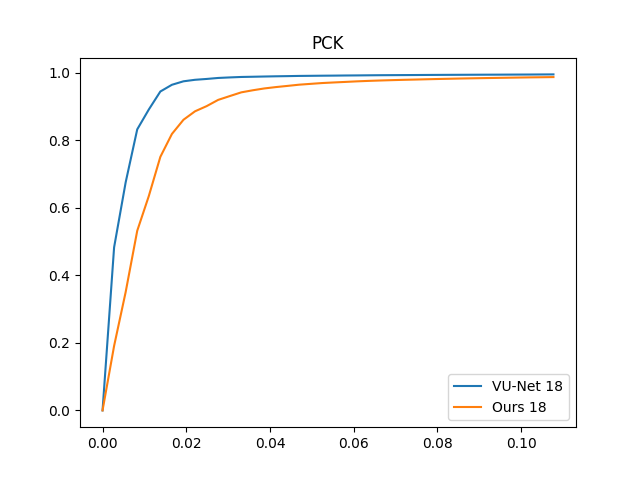
\includegraphics[trim={0cm 0cm 0cm 0cm},clip, width=1.0\linewidth]{fig/pck18}
		% \end{subfigure}
		% \begin{subfigure}{0.49\linewidth}
		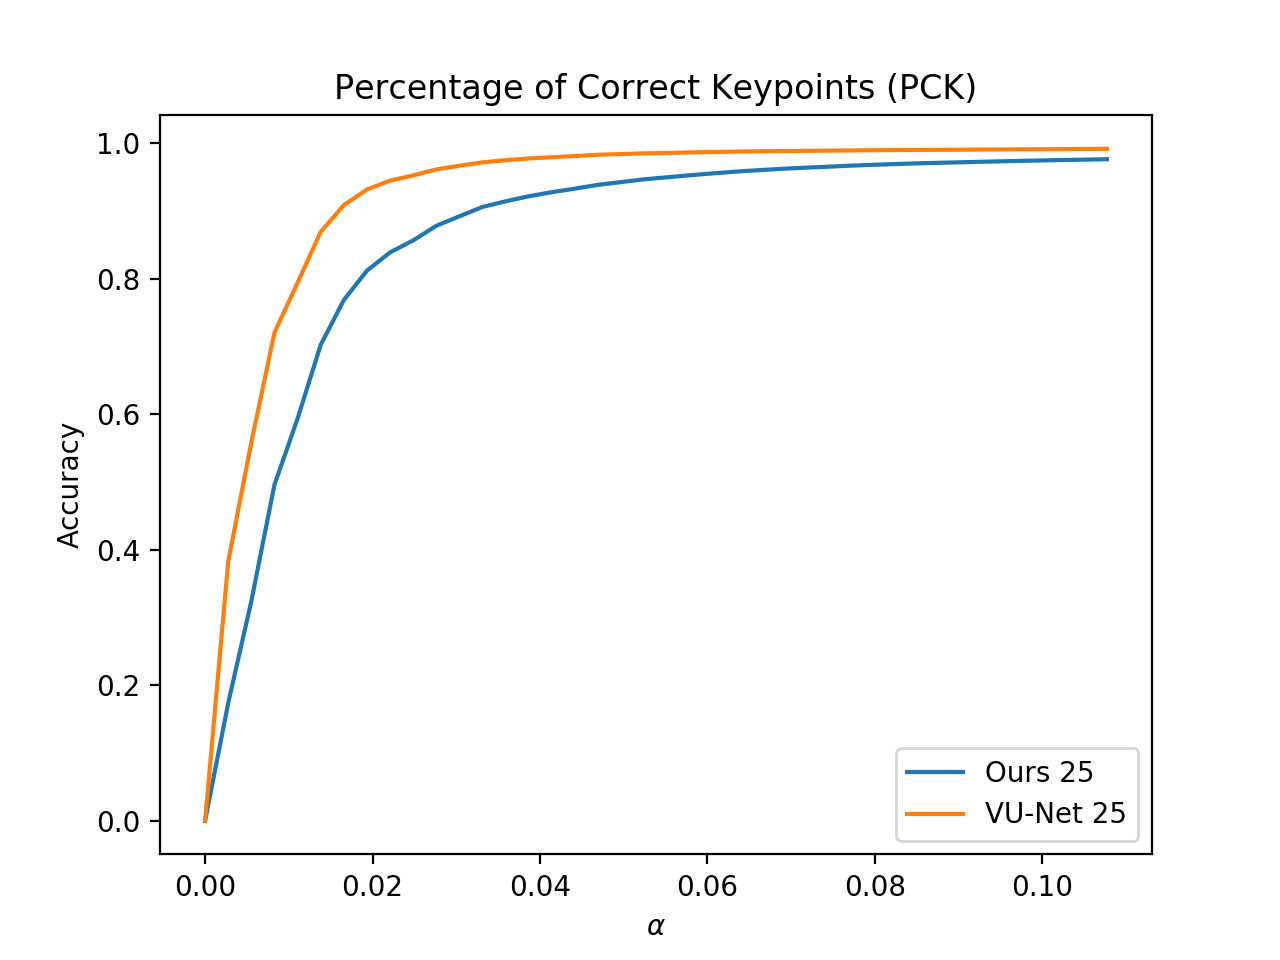
\includegraphics[trim={0cm 0cm 0cm 0cm},clip, width=0.7\linewidth]{fig/factor/pck25}
		% \end{subfigure}
		\caption{PCK Curve for VU-Net \cite{esser18} and Ours for re-estimating pose with a 25 keypoint human pose detector.}
		\label{fig:pckcurve}
	\end{figure}

	To evaluate shape, we extract keypoints using the pose estimator \cite{cao17affinityfield}. Tab. \ref{tab:pose} reports the difference between generated and pose target in percentage of correct keypoints (PCK), Fig. \ref{fig:pckcurve} shows the comparison of PCK curves. As would be expected, VU-Net performs better, since it is trained with exactly the keypoints of \cite{cao17affinityfield}. Still our approach achieves an impressive PCK without supervision underlining the disentanglement of appearance and shape.


	\section{Factorizing into Parts}
	% PART SWAPS
	\begin{figure}[ht]
		\begin{subfigure}{0.49\linewidth}
		\centering
		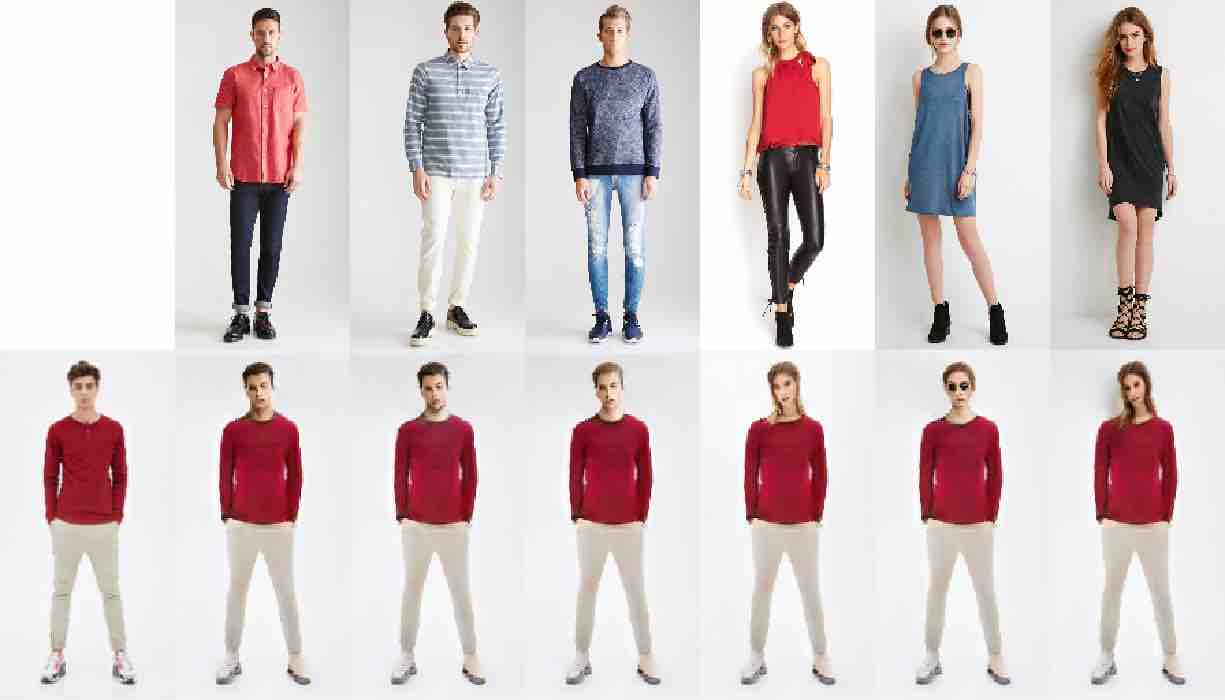
\includegraphics[trim={0cm 0cm 0cm 0cm},clip, width=1.\linewidth]{fig/factor/part6_01}\caption{}
		\label{fig:part3_00}
		\end{subfigure}
		\begin{subfigure}{0.49\linewidth}
		\centering
		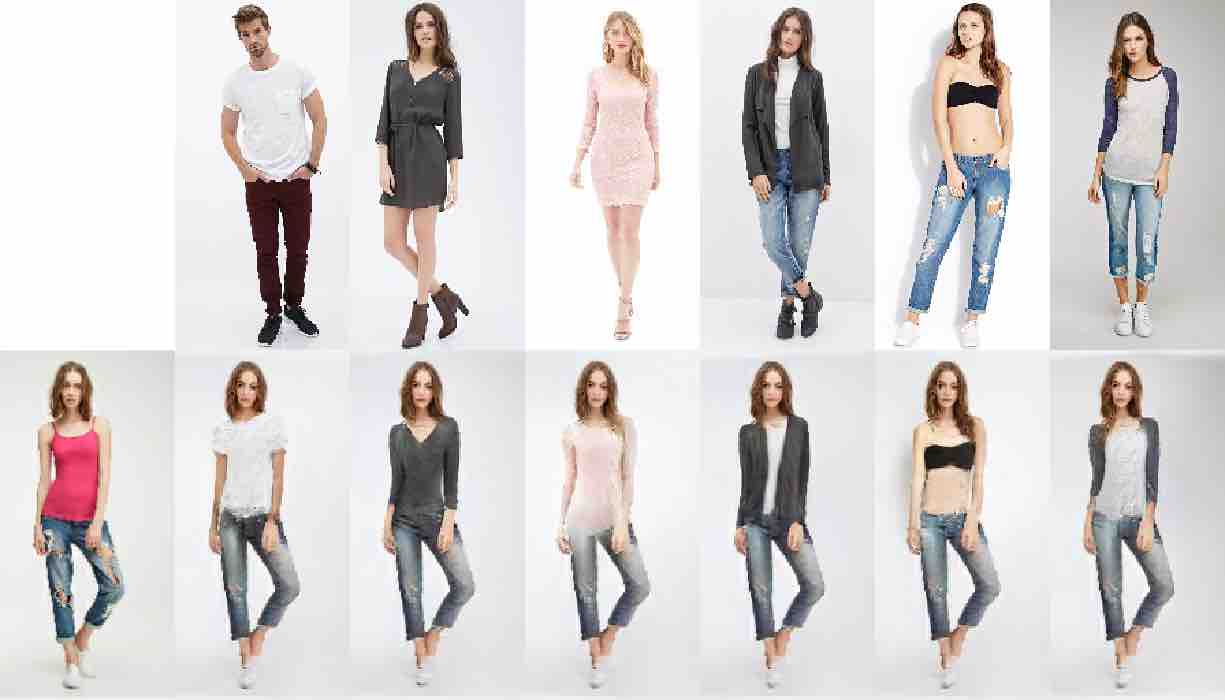
\includegraphics[trim={0cm 0cm 0cm 0cm},clip, width=1.\linewidth]{fig/factor/part6_10}\caption{}
		\label{fig:part3_11}
		\end{subfigure}
		\begin{subfigure}{0.49\linewidth}
		\centering
		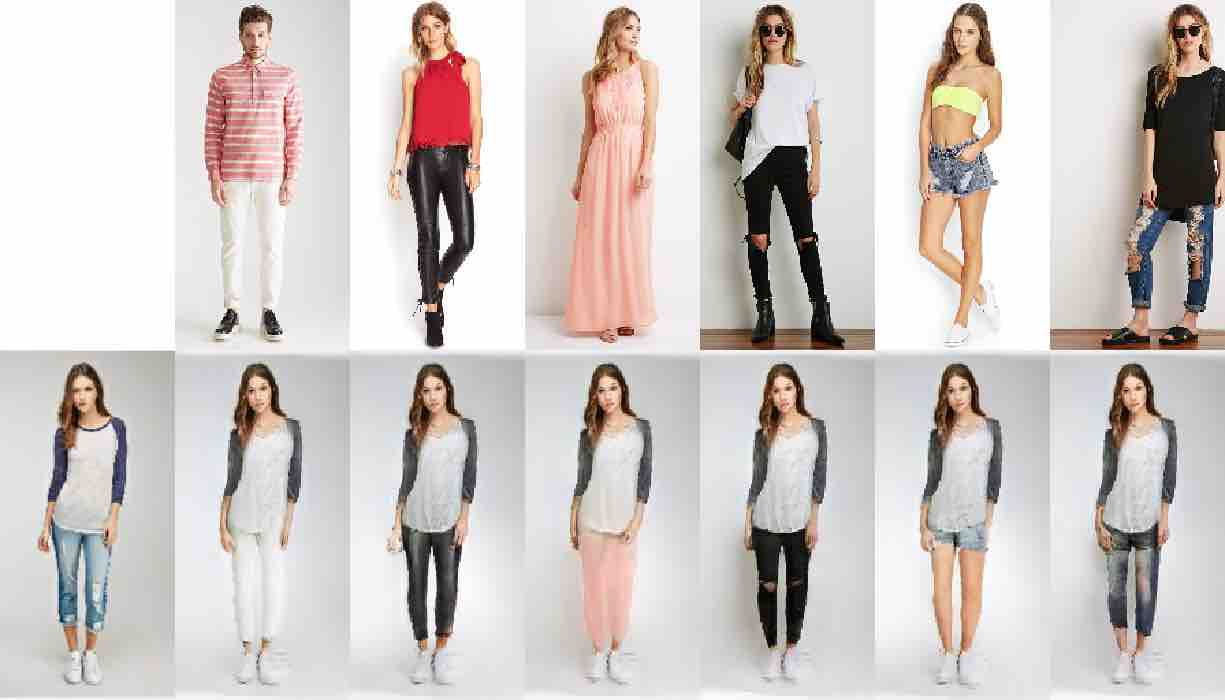
\includegraphics[trim={0cm 0cm 0cm 0cm},clip, width=1.\linewidth]{fig/factor/part6_21}\caption{}
		\label{fig:part3_21}
		\end{subfigure}
		\begin{subfigure}{0.49\linewidth}
		\centering
		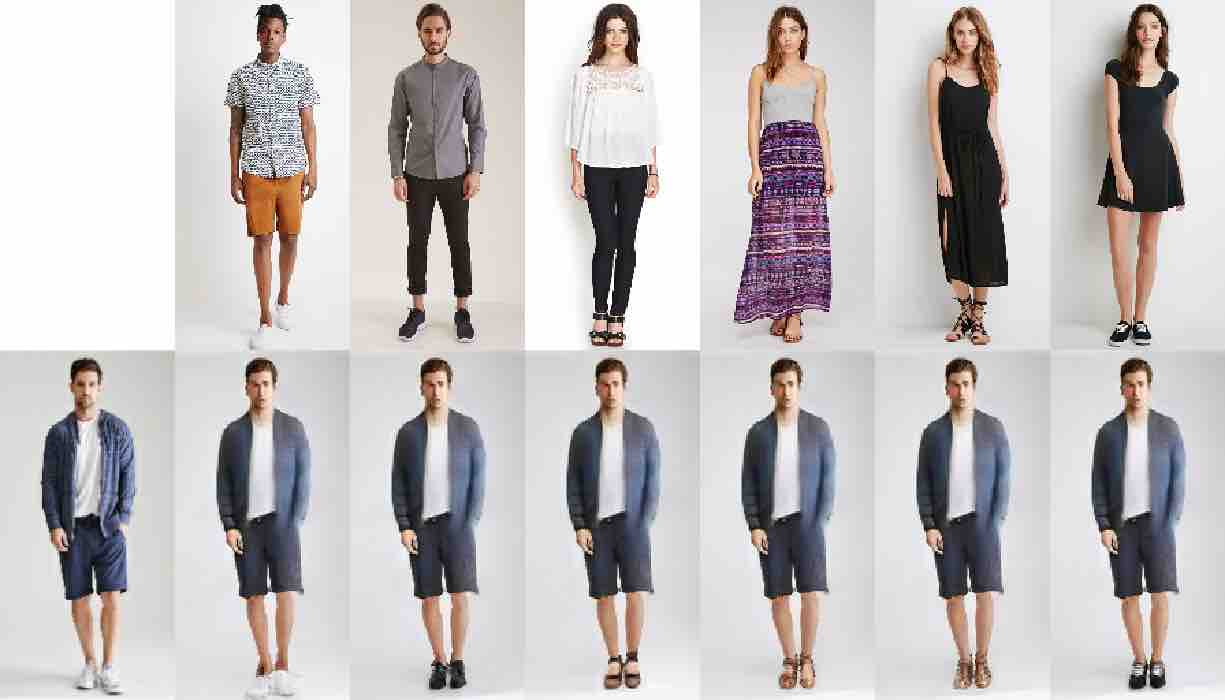
\includegraphics[trim={0cm 0cm 0cm 0cm},clip, width=1.\linewidth]{fig/factor/part6_30}\caption{}
		\label{fig:part3_30}
		\end{subfigure}
		\caption{Swapping part appearance on Deep Fashion. Appearances can be exchanged for parts individually and without altering shape. We show part-wise swaps for (a) head (b) torso (c) legs, (d) shoes. All images are from the test set.}
		\label{fig:partswaps}
	\end{figure}
	\begin{itemize}
		\item Own Dataset: Move KP
		\item DeepFashion: exchange parts
	\end{itemize}

	\begin{figure}[htp]
		\centering
		\begin{subfigure}{1.\linewidth}
		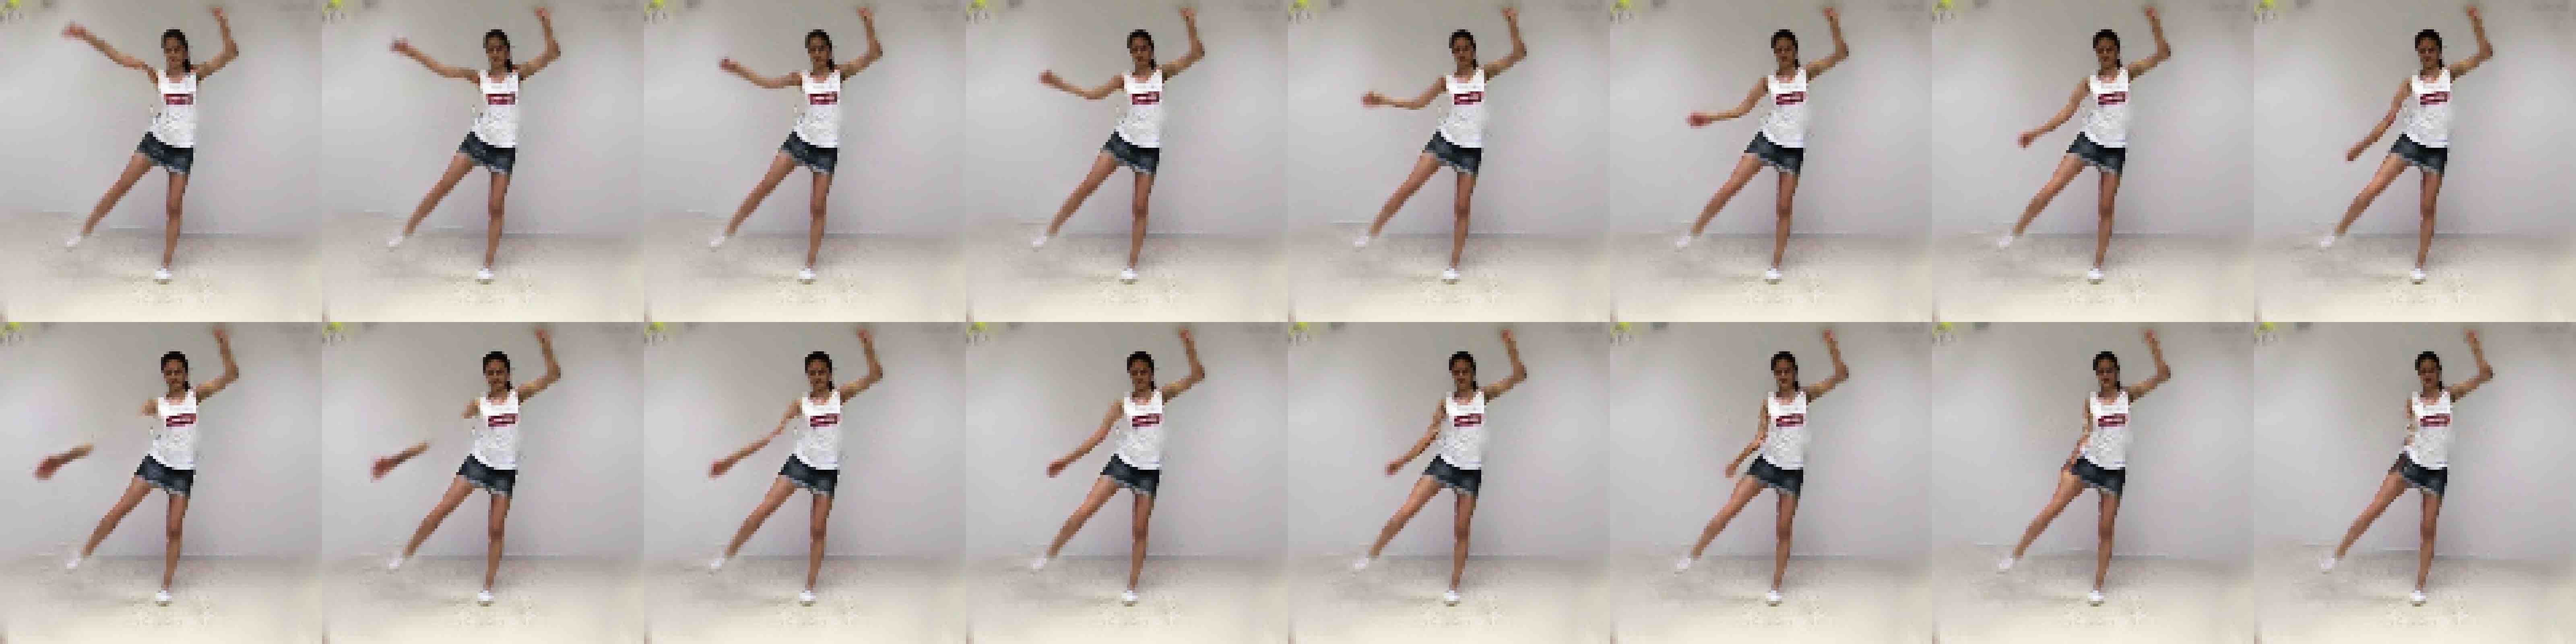
\includegraphics[trim={0cm 0cm 0cm 0cm},clip, width=1.0\linewidth]{fig/factor/8arm}\caption{}
		\end{subfigure}

		\begin{subfigure}{1.\linewidth}
			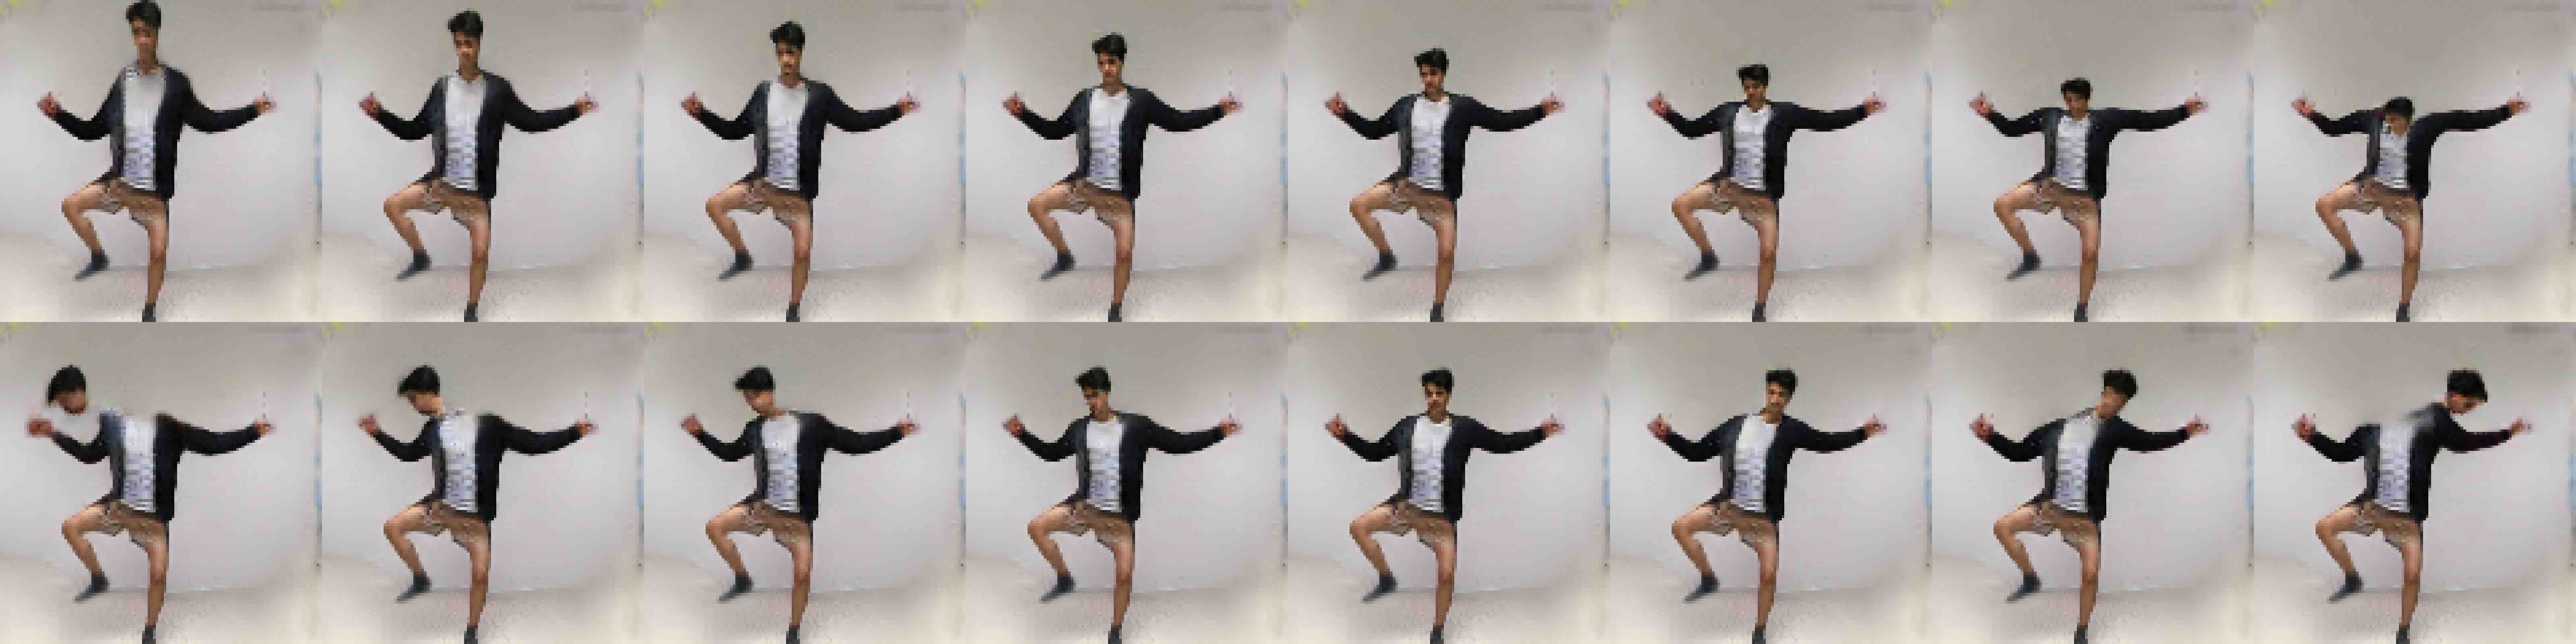
\includegraphics[trim={0cm 0cm 0cm 0cm},clip, width=1.0\linewidth]{fig/factor/8head}\caption{}
		\end{subfigure}
		% \begin{subfigure}{0.8\linewidth}
		% 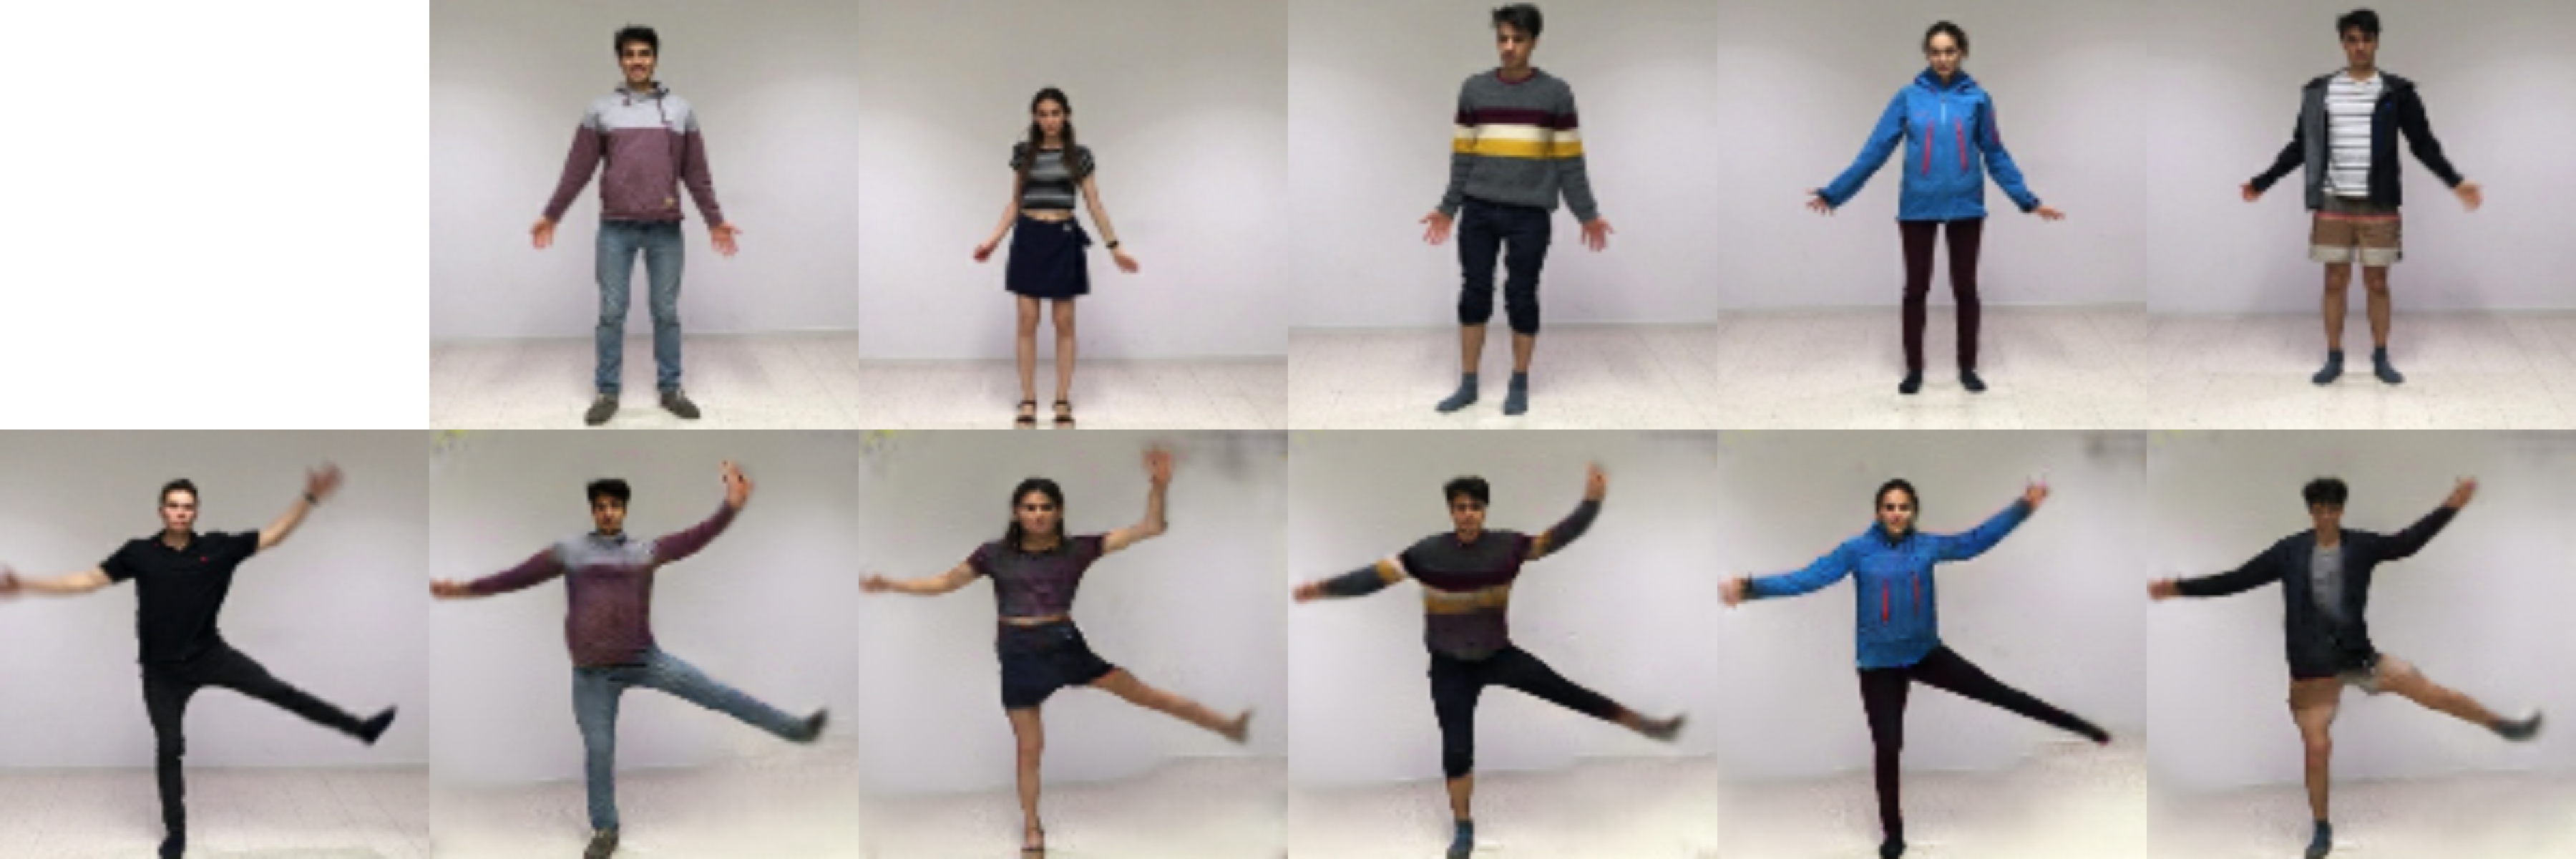
\includegraphics[trim={0cm 0cm 0cm 0cm},clip, width=1.0\linewidth]{fig/factor/app}
		% \end{subfigure}
		\caption{Moving individual body landmarks for conditional generation (a) arm (b) head.}
		\label{fig:movekp}
	\end{figure}

\section{Follow-Up}
	\begin{itemize}
		\item make generative:(KP distribution estimation, variational features).
		\item make video generation possible (RNN on KP vector).
		\item better transformations -> appearance locally (around parts changed), appearance changed perceptually -> style transfer
		\item local appearance change (as TPS)
	\end{itemize}


	% BBC THUMB
	\begin{figure}[t]
		\centering
		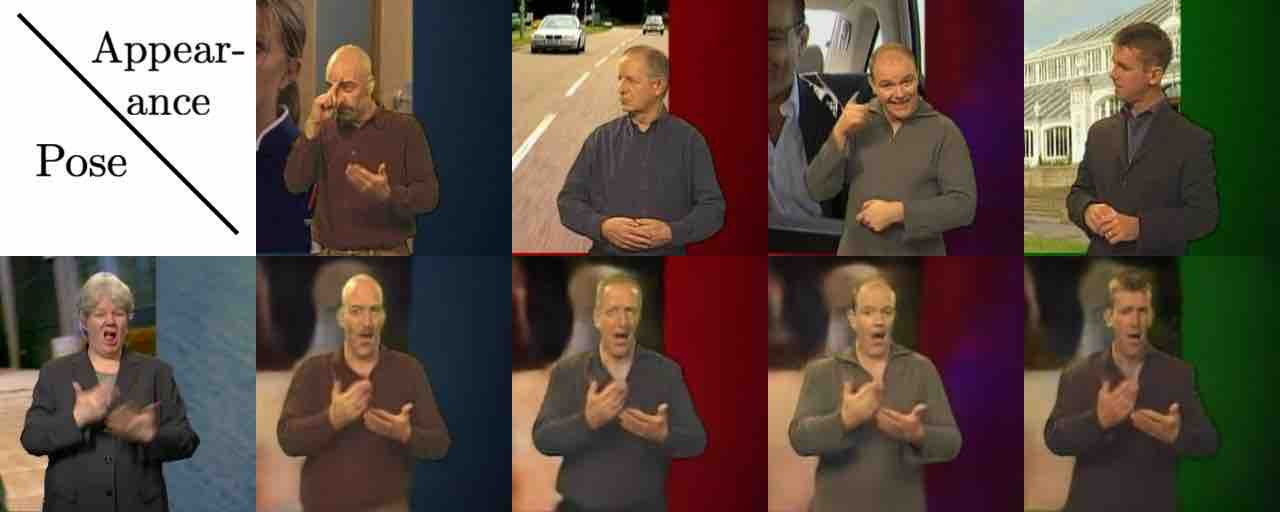
\includegraphics[trim={0cm 0cm 0cm 0cm},clip, width=.7\linewidth]{fig/factor/bbcthumb5}
		\caption{Video-to-video translation on BBC Pose. Top-row: target appearances, left: target pose.
		%The target appearances are from the train set, while the target pose is from the test set.
		Note that even fine details in shape are accurately captured. See supplementary for videos.}
		\label{fig:bbcthumb}
	\end{figure}

